\documentclass[11pt, a4paper]{article}

\usepackage[margin=2.5cm]{geometry}
\usepackage{booktabs}
\usepackage{longtable}
\usepackage{array}
\usepackage{tabularx}
\usepackage{xcolor}
\usepackage{hyperref}
\usepackage{titlesec}
\usepackage{enumitem}
\usepackage{fancyhdr}
\usepackage{amsmath}
\usepackage{amssymb}
\usepackage{microtype}
\usepackage{parskip}
\usepackage{mdframed}
\usepackage{tikz}
\usetikzlibrary{shapes.geometric, arrows.meta, positioning, fit, backgrounds}

% --- colour palette (phosphor green theme) ---
\definecolor{phosphor}{RGB}{20, 200, 20}
\definecolor{dimgreen}{RGB}{10, 120, 10}
\definecolor{darkbg}{RGB}{8, 20, 8}
\definecolor{accentcyan}{RGB}{0, 180, 220}
\definecolor{accentred}{RGB}{220, 40, 20}
\definecolor{tabhead}{RGB}{20, 60, 20}
\definecolor{rowalt}{RGB}{230, 245, 230}
\definecolor{notebg}{RGB}{240, 250, 240}

% --- hyperref ---
\hypersetup{
  colorlinks = true,
  linkcolor  = dimgreen,
  urlcolor   = accentcyan,
  citecolor  = dimgreen,
}

% --- header / footer ---
\pagestyle{fancy}
\fancyhf{}
\fancyhead[L]{\small\textcolor{dimgreen}{OAMP — Development Roadmap}}
\fancyhead[R]{\small\textcolor{dimgreen}{Phases 2 \& 3}}
\fancyfoot[C]{\small\textcolor{dimgreen}{\thepage}}
\renewcommand{\headrulewidth}{0.4pt}
\renewcommand{\headrule}{\hbox to\headwidth{\color{dimgreen}\leaders\hrule height \headrulewidth\hfill}}

% --- section styling ---
\titleformat{\section}{\large\bfseries\color{dimgreen}}{}{0em}{}[\textcolor{dimgreen}{\titlerule[0.6pt]}]
\titleformat{\subsection}{\normalsize\bfseries\color{dimgreen!80!black}}{}{0em}{}
\titleformat{\subsubsection}{\normalsize\itshape\color{dimgreen!70!black}}{}{0em}{}

% --- note box ---
\newmdenv[
  backgroundcolor=notebg,
  linecolor=dimgreen,
  linewidth=1pt,
  leftmargin=0pt, rightmargin=0pt,
  innerleftmargin=10pt, innerrightmargin=10pt,
  innertopmargin=6pt, innerbottommargin=6pt,
]{notebox}

% --- table helpers ---
\newcolumntype{L}[1]{>{\raggedright\arraybackslash}p{#1}}
\newcolumntype{C}[1]{>{\centering\arraybackslash}p{#1}}

\begin{document}

% ============================================================
%  TITLE
% ============================================================
\begin{titlepage}
  \pagecolor{darkbg}
  \color{phosphor}
  \vspace*{3cm}
  \begin{center}
    {\Huge\bfseries Open Source Astrodynamic\\[0.3em]
     Mission Planning}\\[1.5em]
    {\LARGE\color{accentcyan} Development Roadmap}\\[0.8em]
    {\large Phases 2 \& 3}\\[3cm]
    \textcolor{phosphor!60!black}{\rule{0.5\textwidth}{0.4pt}}\\[1em]
    {\normalsize
      Precision Newtonian Mission Design \quad\textbullet\quad
      Post-Newtonian \& General Relativity}\\[2em]
    {\small\color{phosphor!60!black}
      Apache-2.0 \quad|\quad HortDog \quad|\quad \today}
  \end{center}
\end{titlepage}

\pagecolor{white}
\color{black}

% ============================================================
%  TABLE OF CONTENTS
% ============================================================
\tableofcontents
\newpage

% ============================================================
%  EXECUTIVE SUMMARY
% ============================================================
\section{Executive Summary}

Phase~1 delivered the project skeleton: a Newtonian $+$~J2 propagator with
DOP853 integration, an open-loop launch simulator, a SPICE kernel wrapper with
reproducibility-locked manifests, and a WebGPU~3D viewer showing three orbital
scenarios. All 10 unit tests pass; the stack is clean (ruff, TypeScript strict).

\textbf{Phase~2} keeps the physics Newtonian but raises the fidelity to the
level needed for real mission design: higher-order gravity, atmospheric drag,
solar radiation pressure, third-body perturbations, TLE ingest, $\Delta v$
manoeuvre planning, a Lambert/CasADi trajectory optimizer, live WebSocket
streaming, and a full manoeuvre-editor frontend.

\textbf{Phase~3} adds post-Newtonian (PN) corrections and a full General
Relativity (GR) geodesic integrator on the DSX/Brumberg--Kopejkin BCRS metric,
with tetrad thrust modelling and a Ray-backed spacetime metric pre-bake cache
for performance.

\begin{notebox}
\textbf{Convention lock (unchanged from Phase~1):}
UTC ISO-8601 on the wire; TDB seconds since J2000 (= SPICE ET) internally.
All SI units in the engine. Apache-2.0 licence.
\end{notebox}

% ============================================================
%  PHASE 2
% ============================================================
\newpage
\section{Phase 2 — Precision Newtonian \& Mission Design}

\subsection{Goals}

A mission designer should be able to: load a TLE or specify an initial state,
apply atmospheric drag and solar radiation pressure, add impulsive $\Delta v$
burns, solve a Lambert transfer or run a fuel-optimal CasADi optimisation, and
watch the result stream live in the 3D viewer.

\subsection{2a — Dynamics Fidelity}

\subsubsection{Higher-Order Gravity}

Extend \texttt{oamp.dynamics.newtonian} with zonal harmonics $J_3$--$J_6$
(Vallado §8.7). The acceleration from $J_n$ is:

\begin{equation}
  \mathbf{a}_{J_n} = -\frac{\mu}{r^2} \frac{n+1}{2}
    \left(\frac{R_\oplus}{r}\right)^n J_n \,
    \nabla P_n(\sin\phi)
\end{equation}

where $P_n$ is the Legendre polynomial and $\phi$ the geocentric latitude.
Tesseral ($C_{nm}$, $S_{nm}$) terms are planned but deferred to Phase~2b+.

\subsubsection{Atmospheric Drag}

Replace the exponential density model in \texttt{launch.py} with
NRLMSISE-00 via the \texttt{nrlmsise00} Python package. The drag acceleration
is:

\begin{equation}
  \mathbf{a}_\text{drag} = -\tfrac{1}{2}\, \rho(h)\, C_D\, \frac{A}{m}\,
    |\mathbf{v}_\text{rel}|\,\mathbf{v}_\text{rel}
\end{equation}

where $\mathbf{v}_\text{rel}$ accounts for Earth's rotation
($\boldsymbol{\omega}_\oplus \times \mathbf{r}$). Vehicle cross-section $A$
and $C_D$ are added to the propagation request body.

\subsubsection{Solar Radiation Pressure}

Cannonball model with cylindrical shadow cones for Earth and Moon:

\begin{equation}
  \mathbf{a}_\text{SRP} = \nu \frac{P_\odot}{c}
    \frac{A_\text{eff}}{m} \hat{\mathbf{r}}_{\odot}
\end{equation}

where $\nu \in [0,1]$ is the shadow function (computed via SPICE body
positions already available) and $P_\odot = 4.56\times10^{-6}$~N~m$^{-2}$
at 1~AU.

\subsubsection{Third-Body Gravity}

Moon and Sun perturbations using SPICE \texttt{body\_state()} (already
implemented) with point-mass attractions and the indirect term:

\begin{equation}
  \mathbf{a}_\text{3b} = \sum_k \mu_k
    \left(\frac{\mathbf{r}_k - \mathbf{r}}{|\mathbf{r}_k - \mathbf{r}|^3}
          - \frac{\mathbf{r}_k}{|\mathbf{r}_k|^3}\right)
\end{equation}

\subsubsection{Symplectic Integrator}

Add SABA2 (symplectic Birkhoff--Adams) alongside DOP853 for long-arc
propagation where energy conservation over months matters more than step-size
adaptivity. Selectable via \texttt{integrator: "dop853" | "saba2"} in the
request.

\subsubsection{New API Flags}

\begin{center}
\begin{tabular}{L{3cm} L{4cm} L{5cm}}
  \toprule
  \textbf{Field} & \textbf{Type} & \textbf{Effect} \\
  \midrule
  \texttt{drag}       & \texttt{bool}        & NRLMSISE-00 drag \\
  \texttt{srp}        & \texttt{bool}        & Solar radiation pressure \\
  \texttt{third\_body}& \texttt{list[str]}   & Bodies e.g.\ \texttt{["moon","sun"]} \\
  \texttt{jn\_max}    & \texttt{int}         & Max zonal harmonic (2–6) \\
  \texttt{integrator} & \texttt{str}         & \texttt{"dop853"} or \texttt{"saba2"} \\
  \texttt{vehicle}    & \texttt{VehicleModel}& $m$, $A$, $C_D$, $C_R$ \\
  \bottomrule
\end{tabular}
\end{center}

\subsubsection{Tests}

\begin{itemize}[noitemsep]
  \item Energy drift $< 10^{-9}$ relative over 30-day arc (SABA2)
  \item Nodal regression matches NRLMSISE drag prediction within 5\%
  \item SRP produces correct signature in inclination evolution
  \item Moon third-body matches SPICE-derived perturbation to $< 1$~m/day
\end{itemize}

\subsection{2b — TLE Ingest}

Add \texttt{GET /tle?norad=\{id\}} which:
\begin{enumerate}[noitemsep]
  \item Fetches the current TLE from Celestrak
  \item Parses with \texttt{sgp4} (already evaluable from \texttt{conda-forge})
  \item Propagates to epoch via SGP4
  \item Converts mean-element state to osculating Cartesian (Brouwer transform)
  \item Returns an \texttt{InitialState} compatible with \texttt{POST /propagate}
\end{enumerate}

A manifest of pinned test TLEs (NORAD ID + epoch + expected state checksum)
mirrors the SPICE kernel manifest pattern for reproducible CI.

\subsection{2c — $\Delta v$ Manoeuvre Engine}

\subsubsection{Data Model}

\begin{verbatim}
class Maneuver(BaseModel):
    t_tdb: float                # TDB seconds since J2000
    dv_ric: list[float]         # [radial, in-track, cross-track], m/s
\end{verbatim}

\texttt{POST /propagate} accepts an optional \texttt{maneuvers: list[Maneuver]};
the integrator applies instantaneous velocity kicks at each epoch by
transforming RIC $\to$ ECI and restarting the ODE.

\subsubsection{Analytical Solvers}

\begin{center}
\begin{tabular}{L{3.5cm} L{9cm}}
  \toprule
  \textbf{Endpoint} & \textbf{Description} \\
  \midrule
  \texttt{POST /optimize/hohmann}  &
    Closed-form two-impulse Hohmann transfer. Returns $\Delta v_1$,
    $\Delta v_2$, transfer time. \\[4pt]
  \texttt{POST /optimize/lambert}  &
    Universal-variable Lambert solver (Izzo/Gooding algorithm) for
    arbitrary two-point boundary-value transfer. \\
  \bottomrule
\end{tabular}
\end{center}

\subsubsection{Numerical Optimiser}

\texttt{POST /optimize/trajectory} uses CasADi (already in the \texttt{default}
pixi environment) to solve the fuel-optimal NLP:

\begin{equation}
  \min_{\{\Delta \mathbf{v}_k\}} \sum_k |\Delta \mathbf{v}_k|
  \quad \text{s.t.} \quad
  \mathbf{x}_{k+1} = \phi(\mathbf{x}_k + \Delta\mathbf{v}_k,\, \Delta t_k),\;
  \mathbf{x}_N = \mathbf{x}_\text{target}
\end{equation}

The propagation $\phi$ is the DOP853 integrator wrapped as a CasADi callback.
Warm-starting from the Lambert solution typically converges in $< 30$~iterations.

\subsection{2d — Real-time WebSocket Streaming}

Replace the echo-only \texttt{/ws} channel with a streaming propagator. The
protocol uses msgpack (already a dependency):

\begin{enumerate}[noitemsep]
  \item Client sends \texttt{\{scenario\_id, t\_start, t\_end, dt, config\}}
  \item Server propagates in chunks of $N$ steps on a Ray actor (or asyncio for
        small jobs)
  \item Each chunk is msgpack-encoded and sent as a binary WebSocket frame
  \item A terminal \texttt{\{done: true, elapsed\_ms\}} frame closes the stream
\end{enumerate}

This enables the frontend time-scrubber to show live progress for long
multi-day propagations.

\subsection{2e — Frontend}

\begin{center}
\begin{tabularx}{\textwidth}{L{3.5cm} X}
  \toprule
  \textbf{Feature} & \textbf{Detail} \\
  \midrule
  Manoeuvre editor &
    Click on trajectory to insert a burn node; drag the arrow glyph to adjust
    $\Delta v$ magnitude and direction in the RIC frame. \\[4pt]
  Time scrubber &
    Slider replays the trajectory; a spacecraft marker moves along the path.
    Shows $t_\text{UTC}$, $r$, $v$, and remaining $\Delta v$ budget. \\[4pt]
  Multi-trajectory overlay &
    Compare baseline vs optimised trajectories side-by-side with per-trajectory
    colour coding and a difference-norm plot in a side panel. \\[4pt]
  Velocity / thrust vectors &
    Short arrow glyphs at the spacecraft position; length proportional to
    $|\mathbf{v}|$ or $|\mathbf{f}|$ with configurable scale. \\[4pt]
  WebGL2 fallback &
    2D ground-track canvas (equirectangular) for browsers without WebGPU.
    Uses the same trajectory data from the REST API. \\[4pt]
  Scenario save/load &
    JSON export of full mission state (initial conditions, manoeuvres,
    vehicle model, propagation config). Drag-and-drop import. \\
  \bottomrule
\end{tabularx}
\end{center}

\subsection{Phase 2 Sequencing}

\begin{center}
\begin{tabular}{L{5cm} C{2.5cm} L{5.5cm}}
  \toprule
  \textbf{Work item} & \textbf{Est.\ duration} & \textbf{Dependency} \\
  \midrule
  2a Drag + third-body     & 2--3 weeks & Phase 1 \\
  2b TLE ingest            & 1 week     & Phase 1 \\
  2c Lambert + CasADi NLP  & 2--3 weeks & 2a \\
  2d WebSocket streaming   & 1 week     & Phase 1 \\
  2e Frontend              & 3--4 weeks & 2c, 2d (parallel) \\
  \midrule
  \textbf{Total}           & \textbf{9--12 weeks} & \\
  \bottomrule
\end{tabular}
\end{center}

% ============================================================
%  PHASE 3
% ============================================================
\newpage
\section{Phase 3 — Post-Newtonian \& General Relativity}

\subsection{Goals}

Provide GR-fidelity propagation for precision science missions: geodetic
surveying, pulsar timing, deep-space navigation, and any scenario where
Newtonian errors exceed the mission budget. The Newtonian path remains the
fast default; GR is opt-in via \texttt{physics: "pn1" | "gr"}.

\subsection{3a — Post-Newtonian Corrections (Bridge Layer)}

PN corrections are additive accelerations on top of the existing DOP853
integrator — no new integrator required. This makes validation straightforward:
the PN limit must reproduce known analytic results before the full GR engine
is trusted.

\subsubsection{Schwarzschild (1PN)}

The dominant solar-system GR effect. In isotropic coordinates:

\begin{equation}
  \mathbf{a}_\text{Schw} = \frac{\mu}{c^2 r^3}
  \left[
    \left(4\frac{\mu}{r} - v^2\right)\mathbf{r}
    + 4(\mathbf{r}\cdot\mathbf{v})\mathbf{v}
  \right]
\end{equation}

\subsubsection{Lense--Thirring (1PN Frame-Dragging)}

Spin--orbit coupling from Earth's angular momentum
$\mathbf{S} = I_\oplus \boldsymbol{\omega}_\oplus$:

\begin{equation}
  \mathbf{a}_\text{LT} = \frac{2G}{c^2 r^3}
  \left[
    \left(\frac{\mathbf{r}}{r}\times\mathbf{v}\right)\times\mathbf{S}
    + \frac{3}{r^2}\left(\mathbf{S}\cdot\mathbf{r}\right)
      \left(\mathbf{r}\times\mathbf{v}\right)
  \right]
\end{equation}

\subsubsection{de~Sitter / Geodetic Precession (1PN)}

Solar barycentric contribution to orbit precession:

\begin{equation}
  \boldsymbol{\Omega}_\text{dS} =
    \frac{3}{2}\frac{GM_\odot}{c^2 a_\oplus(1-e_\oplus^2)}
    \frac{\boldsymbol{n}_\oplus \times \mathbf{v}_\oplus}{|\mathbf{v}_\oplus|}
\end{equation}

\subsubsection{Validation Tests}

\begin{itemize}[noitemsep]
  \item Mercury perihelion precession: $42.98''$/century $\pm\,0.5\%$
  \item Gravity Probe~B geodetic precession: $6606.1\,$mas/yr $\pm\,1\%$
  \item Shapiro delay signature reproduced for Earth--Moon baseline
  \item PN accelerations vanish in the $c\to\infty$ limit (numerical check)
\end{itemize}

\subsection{3b — Full GR Geodesic Integrator}

\subsubsection{Metric}

DSX metric / Brumberg--Kopejkin Barycentric Celestial Reference System (BCRS).
For a test particle of negligible mass the line element is:

\begin{equation}
  ds^2 = -\left(1 - \frac{2w}{c^2}\right)c^2\,dt^2
         + \left(1 + \frac{2w}{c^2}\right)\delta_{ij}\,dx^i\,dx^j
         + \mathcal{O}(c^{-4})
\end{equation}

where $w = \sum_A G M_A / r_A$ is the Newtonian potential summed over all
Solar-system bodies $A$.

\subsubsection{State Vector}

\begin{equation}
  \mathbf{X} = \bigl(t_\text{TDB},\; x^\mu,\; u^\mu\bigr)
  \quad\in\quad \mathbb{R}^{1+4+4}
\end{equation}

with the constraint $g_{\mu\nu} u^\mu u^\nu = -c^2$ monitored as an invariant.

\subsubsection{Equations of Motion}

Geodesic equation with optional non-geodesic thrust $f^\alpha$:

\begin{equation}
  \frac{Du^\alpha}{d\tau}
  = \frac{du^\alpha}{d\tau}
    + \Gamma^\alpha{}_{\mu\nu}\, u^\mu u^\nu
  = f^\alpha
\end{equation}

Christoffel symbols $\Gamma^\alpha{}_{\mu\nu}$ are computed analytically from
the PN metric expansion (no numerical differentiation).

\subsubsection{Integrator}

DOP853 on the 8D geodesic state with adaptive step-size; fallback to a
symplectic Runge--Kutta--Nyström for long arcs. The norm constraint
$g_{\mu\nu}u^\mu u^\nu + c^2$ is logged as a quality indicator.

\subsubsection{Endpoint}

\texttt{POST /propagate/gr} — accepts BCRS initial conditions in SI plus
coordinate time span. Returns proper time $\tau$, coordinate trajectory
$x^\mu(\tau)$, and the 4-velocity $u^\mu(\tau)$.

\subsection{3c — Tetrad Thrust Model}

Converts coordinate-frame thrust commands to the local orthonormal tetrad:

\begin{enumerate}[noitemsep]
  \item Build tetrad $e^\mu{}_{(a)}$ from $u^\mu$ and the spacecraft attitude
  \item Decompose thrust in the tetrad frame:
        $f^\alpha = (f^{\hat{0}}, f^{\hat{1}}, f^{\hat{2}}, f^{\hat{3}})$
  \item Inject as right-hand side of the non-geodesic equation above
\end{enumerate}

\texttt{POST /propagate/gr} accepts \texttt{thrust\_tetrad\_N: [float, float, float]}
(body-frame thrust in Newtons; frame defined relative to $u^\mu$ and a
reference attitude quaternion).

\subsection{3d — Multi-body Metric Pre-bake (Ray Workers)}

\subsubsection{Motivation}

Evaluating the BCRS metric and its derivatives at every integration step for
every Solar-system body at full SPICE fidelity is the dominant cost of GR
propagation (${\sim}100\times$ slower than Newtonian). Pre-baking the metric
on a 4D grid eliminates repeated SPICE calls.

\subsubsection{Implementation}

\begin{enumerate}[noitemsep]
  \item A Ray actor pool (\texttt{metric\_build}) samples $w(\mathbf{r}, t)$
        and its spatial gradients on a Cartesian grid over the mission window
  \item Results stored as HDF5 in \texttt{data/metric\_cache/} with a
        SHA256 manifest (same pattern as SPICE kernels)
  \item The GR integrator interpolates bilinearly in space and linearly in time
        — typically ${\lesssim}100\,\mu$s per step vs ${\sim}10$~ms for live SPICE
\end{enumerate}

\begin{verbatim}
pixi run -e full build-metric \
  --start 2025-01-01 --end 2025-06-01 \
  --bodies earth,moon,sun,jupiter \
  --resolution-km 500
\end{verbatim}

\subsubsection{Cache Invalidation}

The manifest pins the SPICE kernel SHA256 hashes used during pre-bake. If any
kernel is updated the cache is considered stale and must be rebuilt.

\subsection{3e — Frontend}

\begin{center}
\begin{tabularx}{\textwidth}{L{3.5cm} X}
  \toprule
  \textbf{Feature} & \textbf{Detail} \\
  \midrule
  GR vs PN vs Newton &
    Three overlaid trajectories, colour-coded, rendered simultaneously.
    Toggle any layer on/off. \\[4pt]
  Residual panel &
    Side panel showing $|\mathbf{r}_\text{GR} - \mathbf{r}_\text{Newton}|$
    vs time; highlights when GR corrections exceed a user-set threshold. \\[4pt]
  Proper time display &
    Elapsed proper time $\tau$ alongside coordinate time $t$ in the HUD;
    shows the integrated gravitational + kinematic time dilation. \\[4pt]
  Metric visualiser &
    2D equatorial slice of the Newtonian potential $w(\mathbf{r})$ as a
    heatmap underlay in the 3D view; toggled via a button. \\
  \bottomrule
\end{tabularx}
\end{center}

\subsection{Phase 3 Sequencing}

\begin{center}
\begin{tabular}{L{5cm} C{2.5cm} L{5.5cm}}
  \toprule
  \textbf{Work item} & \textbf{Est.\ duration} & \textbf{Dependency} \\
  \midrule
  3a PN corrections        & 2 weeks    & Phase 2 \\
  3b GR geodesic integrator& 3--4 weeks & 3a \\
  3c Tetrad thrust model   & 1 week     & 3b \\
  3d Ray metric cache      & 2--3 weeks & 3b \\
  3e Frontend              & 2 weeks    & 3b (parallel with 3d) \\
  \midrule
  \textbf{Total}           & \textbf{10--12 weeks} & \\
  \bottomrule
\end{tabular}
\end{center}

% ============================================================
%  OVERALL TIMELINE
% ============================================================
\newpage
\section{Overall Timeline}

\begin{center}
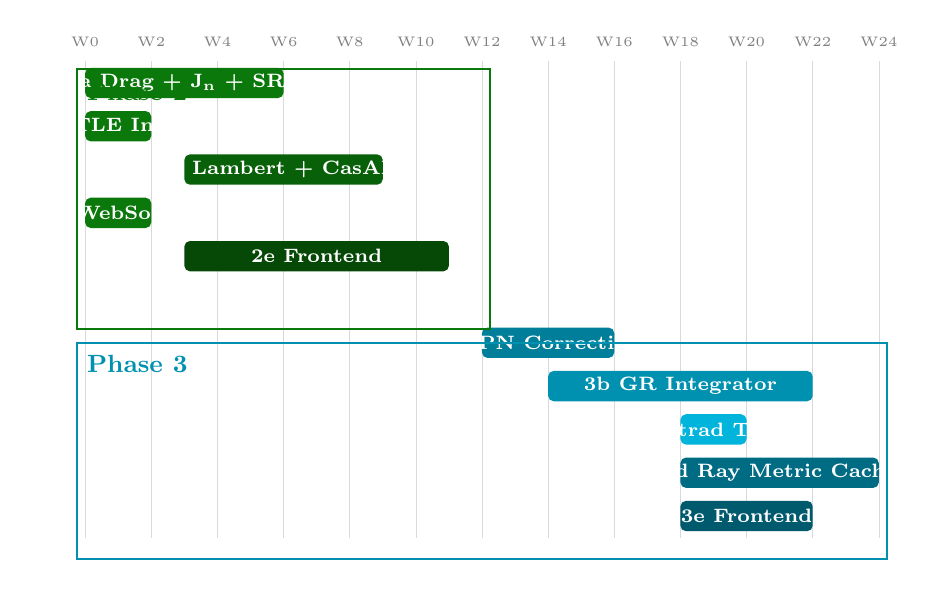
\begin{tikzpicture}[
  bar/.style={rectangle, rounded corners=2pt, minimum height=10pt, text=white,
              font=\scriptsize\bfseries, inner xsep=4pt},
  label/.style={font=\scriptsize, anchor=west},
  week/.style={font=\tiny, color=gray},
]
  \def\W{0.42} % cm per week
  \def\H{0.55} % row height cm

  % --- grid ---
  \foreach \w in {0,2,...,24} {
    \draw[gray!30, very thin] (\w*\W, 0) -- (\w*\W, -11*\H);
    \node[week] at (\w*\W, 0.25) {W\w};
  }

  % Phase 2 bars
  \foreach \row/\start/\len/\col/\txt in {
    1/0/3/dimgreen/{2a Drag + J\textsubscript{n} + SRP},
    2/0/1/dimgreen/{2b TLE Ingest},
    3/3/3/dimgreen!80!black/{2c Lambert + CasADi},
    4/0/1/dimgreen/{2d WebSocket},
    5/3/4/dimgreen!60!black/{2e Frontend}
  } {
    \fill[\col, bar] (\start*\W, -\row*\H+\H*0.15)
      rectangle (\start*\W+\len*\W*2, -\row*\H+\H*0.85)
      node[midway] {\txt};
  }

  % Phase 3 bars
  \foreach \row/\start/\len/\col/\txt in {
    7/12/2/accentcyan!70!black/{3a PN Corrections},
    8/14/4/accentcyan!80!black/{3b GR Integrator},
    9/18/1/accentcyan/{3c Tetrad Thrust},
    10/18/3/accentcyan!60!black/{3d Ray Metric Cache},
    11/18/2/accentcyan!50!black/{3e Frontend}
  } {
    \fill[\col, bar] (\start*\W, -\row*\H+\H*0.15)
      rectangle (\start*\W+\len*\W*2, -\row*\H+\H*0.85)
      node[midway, text=white] {\txt};
  }

  % Phase labels
  \draw[dimgreen, thick] (-0.1, -0.1) rectangle (12*\W+0.1, -6*\H-0.1);
  \node[dimgreen, font=\small\bfseries, anchor=north west] at (-0.1, -0.15)
    {Phase 2};
  \draw[accentcyan!80!black, thick] (-0.1, -6.5*\H) rectangle (24*\W+0.1, -11.5*\H);
  \node[accentcyan!80!black, font=\small\bfseries, anchor=north west]
    at (-0.1, -6.55*\H) {Phase 3};

\end{tikzpicture}
\end{center}

\vspace{1em}

\begin{center}
\begin{tabular}{L{4cm} C{2.5cm} C{2.5cm} C{2.5cm}}
  \toprule
  & \textbf{Phase 1} & \textbf{Phase 2} & \textbf{Phase 3} \\
  \midrule
  Physics model    & Newton + J2     & Newton + J2--J6 + drag + SRP + 3B
                                     & PN + full GR \\
  Integrator       & DOP853          & DOP853 + SABA2  & DOP853 + RKN \\
  Optimiser        & ---             & Lambert + CasADi NLP & CasADi + JAX \\
  Heavy compute    & ---             & Ray (streaming)  & Ray (metric bake) \\
  Frontend         & 3 demo scenes   & Manoeuvre editor + scrubber
                                     & GR/PN/Newton compare \\
  Estimated effort & \emph{done}     & 9--12 weeks     & 10--12 weeks \\
  \bottomrule
\end{tabular}
\end{center}

% ============================================================
%  CONVENTIONS REFERENCE
% ============================================================
\section{Conventions Reference}

\begin{center}
\begin{tabularx}{\textwidth}{L{3cm} X}
  \toprule
  \textbf{Convention} & \textbf{Value} \\
  \midrule
  Licence        & Apache-2.0 (explicit patent grant) \\
  Time on wire   & UTC ISO-8601 string \\
  Time internal  & TDB seconds since J2000 (= SPICE ET); see \texttt{oamp.timescales} \\
  Units          & SI throughout the engine (m, m/s, kg, s) \\
  Accelerator    & JAX (pixi \texttt{gpu} feature); CPU default \\
  Heavy compute  & Ray (pixi \texttt{full} feature) \\
  SPICE kernels  & Pinned by SHA256 in \texttt{backend/oamp/spice/manifest.toml} \\
  Epoch J2000    & 2000-01-01T11:58:55.816Z UTC \\
  $TT - TAI$     & $32.184\,$s (fixed by IAU) \\
  \bottomrule
\end{tabularx}
\end{center}

\end{document}
